% ResonantBERT v3 architecture figure (ACL two-column, full text width = 16 cm).
% Build:  pdflatex architecture.tex   ->  architecture.pdf
% Use:    \begin{figure*}[t]\centering
%           \includegraphics[width=\textwidth]{figures/architecture.pdf}
%           \caption{...}\label{fig:architecture}\end{figure*}
% Drawn at final size: text is 7-9 pt when included at \textwidth.
\documentclass[tikz,border=1pt]{standalone}
\usepackage[T1]{fontenc}
\usepackage{times}
\usepackage{amsmath,amssymb}
\usetikzlibrary{arrows.meta,calc,decorations.pathreplacing}

% Okabe-Ito palette (colour-blind safe); hue encodes role, not section
\definecolor{encC}{HTML}{3B4A63}   % shared encoder
\definecolor{hdC}{HTML}{CC79A7}    % headline segment
\definecolor{bdC}{HTML}{56B4E9}    % body segment
\definecolor{tokC}{HTML}{E69F00}   % token-level heads
\definecolor{segC}{HTML}{009E73}   % segment-level heads
\definecolor{lossC}{HTML}{D55E00}  % training losses
\definecolor{auxC}{HTML}{6A6A6A}   % training-only / ablation

\newcommand{\fA}{\fontsize{9}{10.4}\selectfont}
\newcommand{\fB}{\fontsize{8}{9.2}\selectfont}
\newcommand{\fC}{\fontsize{7}{8.1}\selectfont}
\newcommand{\vb}[1]{\mathbf{#1}}
\newcommand{\Lo}[1]{\mathcal{L}_{\mathrm{#1}}}

\tikzset{
  >={Stealth[length=3.4pt,width=2.8pt]},
  dsh/.style={dash pattern=on 2.2pt off 1.4pt},
  base/.style={rounded corners=1.5pt, line width=0.55pt, align=center, inner sep=1.8pt, font=\fB},
  enc/.style={base, draw=encC, fill=encC!9},
  tok/.style={base, draw=tokC!80!black, fill=tokC!16},
  seg/.style={base, draw=segC!80!black, fill=segC!14},
  aux/.style={base, draw=auxC, dsh, fill=white},
  abl/.style={base, draw=auxC, dotted, line width=0.75pt, fill=white},
  arr/.style={->, line width=0.55pt, draw=black!80},
  auxarr/.style={->, line width=0.55pt, draw=auxC, dsh},
  ablarr/.style={->, line width=0.75pt, draw=auxC, dotted},
  lossarr/.style={->, line width=0.5pt, draw=lossC, dsh},
  loss/.style={font=\fC, text=lossC, align=center, inner sep=1pt},
  note/.style={font=\fC, text=black!70, align=center, inner sep=1pt},
  hdr/.style={font=\fA\bfseries, anchor=base},
  tkn/.style={rounded corners=1pt, line width=0.4pt, minimum width=0.62cm,
              minimum height=0.34cm, inner sep=0pt, font=\fC},
  head/.style={minimum width=1.8cm, minimum height=0.34cm, inner sep=0pt},
}

% \ordinal{y}{expected level in [0,5]}{colour}: five CORAL threshold cells
\newcommand{\ordinal}[3]{%
  \foreach \k in {0,...,4}{%
    \pgfmathsetmacro{\xa}{10.15+\k*0.195}%
    \pgfmathsetmacro{\w}{max(0,min(1,#2-\k))*0.165}%
    \fill[#3] (\xa,#1-0.1) rectangle ++(\w,0.2);%
    \draw[#3!75!black, line width=0.35pt] (\xa,#1-0.1) rectangle ++(0.165,0.2);%
  }%
  \node[note, anchor=west, text=black] at (11.12,#1) {#2};%
}

\begin{document}
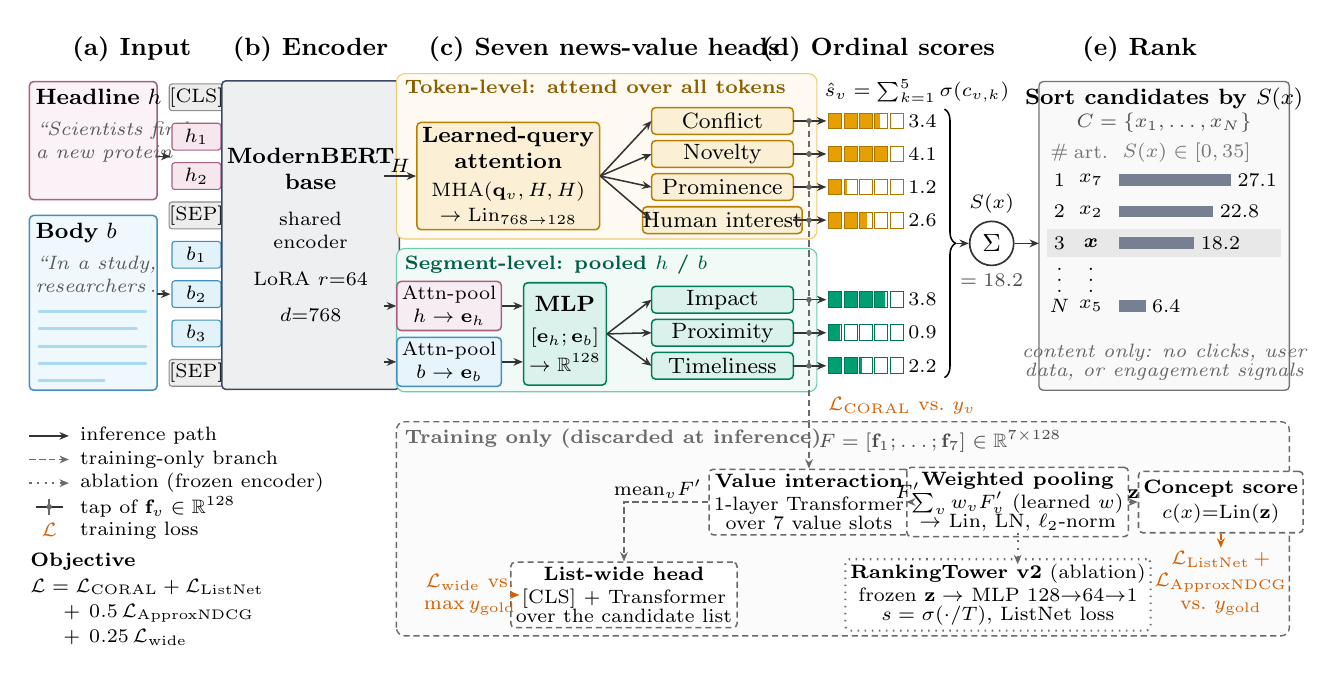
\begin{tikzpicture}[x=1cm, y=1cm, font=\fB]

% ---------------------------------------------------------------- headers
\node[hdr] at (1.30,4.95) {(a) Input};
\node[hdr] at (3.57,4.95) {(b) Encoder};
\node[hdr] at (7.30,4.95) {(c) Seven news-value heads};
\node[hdr] at (10.78,4.95) {(d) Ordinal scores};
\node[hdr] at (14.10,4.95) {(e) Rank};

% ---------------------------------------------------------------- (a) input
\draw[hdC!80!black, fill=hdC!10, line width=0.55pt, rounded corners=1.5pt] (0,3.12) rectangle (1.62,4.62);
\node[anchor=north west, align=left, inner sep=0pt] at (0.07,4.53)
  {\textbf{Headline} $h$\\[2pt]{\fC\itshape\color{black!65}``Scientists find}\\[-1pt]{\fC\itshape\color{black!65}a new protein''}};
\draw[bdC!80!black, fill=bdC!10, line width=0.55pt, rounded corners=1.5pt] (0,0.70) rectangle (1.62,2.92);
\node[anchor=north west, align=left, inner sep=0pt] at (0.07,2.83)
  {\textbf{Body} $b$\\[2pt]{\fC\itshape\color{black!65}``In a study,}\\[-1pt]{\fC\itshape\color{black!65}researchers\,\ldots}};
\foreach \y/\l in {1.70/1.48, 1.48/1.36, 1.26/1.48, 1.04/1.48, 0.82/0.95}
  \draw[bdC!50, line width=1.0pt, line cap=round] (0.12,\y) -- (\l,\y);

% tokenised sequence  [CLS] h [SEP] b [SEP]
\foreach \t/\y/\c in {{[CLS]}/4.42/black, {[SEP]}/2.92/black, {[SEP]}/0.92/black}
  \node[tkn, draw=black!45, fill=black!7] at (2.12,\y) {\t};
\foreach \t/\y in {{$h_1$}/3.92, {$h_2$}/3.42}
  \node[tkn, draw=hdC!80!black, fill=hdC!18] at (2.12,\y) {\t};
\foreach \t/\y in {{$b_1$}/2.42, {$b_2$}/1.92, {$b_3$}/1.42}
  \node[tkn, draw=bdC!80!black, fill=bdC!18] at (2.12,\y) {\t};
\draw[arr] (1.62,3.67) -- (1.79,3.67);
\draw[arr] (1.62,1.92) -- (1.79,1.92);
\foreach \y in {4.42,3.92,3.42,2.92,2.42,1.92,1.42,0.92}
  \draw[arr] (2.44,\y) -- (2.64,\y);

% ---------------------------------------------------------------- (b) encoder
\node[enc, minimum width=1.86cm, minimum height=3.92cm] (enc) at (3.57,2.67)
  {\textbf{ModernBERT}\\\textbf{base}\\[4pt]{\fC shared}\\[-1pt]{\fC encoder}\\[4pt]{\fC LoRA $r{=}64$}\\[4pt]{\fC $d{=}768$}};

% ---------------------------------------------------------------- (c) heads
% token-level lane
\fill[tokC!5, rounded corners=3pt] (4.66,2.62) rectangle (10.0,4.72);
\draw[tokC!55, line width=0.4pt, rounded corners=3pt] (4.66,2.62) rectangle (10.0,4.72);
\node[anchor=north west, font=\fC\bfseries, text=tokC!60!black, inner sep=0pt] at (4.76,4.64)
  {Token-level: attend over all tokens};
\node[tok, minimum width=2.32cm, minimum height=1.30cm] (tq) at (6.08,3.42)
  {\textbf{Learned-query}\\\textbf{attention}\\[1pt]{\fC$\mathrm{MHA}(\vb q_v, H, H)$}\\{\fC$\to\mathrm{Lin}_{768\to128}$}};
\draw[arr] (4.50,3.42) -- node[above, font=\fC, inner sep=1pt] {$H$} (tq.west);

% segment-level lane
\fill[segC!5, rounded corners=3pt] (4.66,0.68) rectangle (10.0,2.50);
\draw[segC!55, line width=0.4pt, rounded corners=3pt] (4.66,0.68) rectangle (10.0,2.50);
\node[anchor=north west, font=\fC\bfseries, text=segC!60!black, inner sep=0pt] at (4.76,2.42)
  {Segment-level: pooled $h$ / $b$};
\node[base, draw=hdC!80!black, fill=hdC!14, minimum width=1.05cm, minimum height=0.58cm] (ph) at (5.33,1.77)
  {{\fC Attn-pool}\\[-1pt]{\fC $h\to\vb e_h$}};
\node[base, draw=bdC!80!black, fill=bdC!14, minimum width=1.05cm, minimum height=0.58cm] (pb) at (5.33,1.06)
  {{\fC Attn-pool}\\[-1pt]{\fC $b\to\vb e_b$}};
\draw[arr] (4.50,1.77) -- (ph.west);
\draw[arr] (4.50,1.06) -- (pb.west);
\node[seg, minimum width=1.05cm, minimum height=1.30cm] (mlp) at (6.80,1.415)
  {\textbf{MLP}\\[2pt]{\fC$[\vb e_h;\vb e_b]$}\\[1pt]{\fC$\to\mathbb{R}^{128}$}};
\draw[arr] (ph.east) -- (ph.east -| mlp.west);
\draw[arr] (pb.east) -- (pb.east -| mlp.west);

% head chips, value scores (example article), taps to the training branch
\draw[auxC, line width=0.55pt, dsh] (9.90,4.12) -- (9.90,0.30);
\foreach \n/\y/\s in {Conflict/4.12/3.4, Novelty/3.70/4.1, Prominence/3.28/1.2, Human interest/2.86/2.6}{
  \node[tok, head] at (8.80,\y) {\n};
  \draw[arr] (tq.east) -- (7.90,\y);
  \draw[arr] (9.70,\y) -- (10.12,\y);
  \fill[auxC] (9.90,\y) circle (1.0pt);
  \ordinal{\y}{\s}{tokC}
}
\foreach \n/\y/\s in {Impact/1.85/3.8, Proximity/1.43/0.9, Timeliness/1.01/2.2}{
  \node[seg, head] at (8.80,\y) {\n};
  \draw[arr] (mlp.east) -- (7.90,\y);
  \draw[arr] (9.70,\y) -- (10.12,\y);
  \fill[auxC] (9.90,\y) circle (1.0pt);
  \ordinal{\y}{\s}{segC}
}

% ---------------------------------------------------------------- (d) ordinal scores
\node[note, text=black, anchor=west] at (10.06,4.50) {$\hat s_v=\sum_{k=1}^{5}\sigma(c_{v,k})$};
\node[loss, anchor=west] at (10.10,0.50) {$\Lo{CORAL}$ vs.\ $y_v$};
\draw[decorate, decoration={brace, amplitude=4pt}, line width=0.55pt] (11.62,4.27) -- (11.62,0.86);
\node[circle, draw=black!80, line width=0.6pt, fill=white, minimum size=0.56cm, inner sep=0pt, font=\fA] (sum) at (12.22,2.565) {$\Sigma$};
\draw[arr] (11.78,2.565) -- (sum.west);
\node[note, text=black, anchor=south] at (12.22,2.90) {$S(x)$};
\node[note, anchor=north] at (12.22,2.22) {$=18.2$};

% ---------------------------------------------------------------- (e) rank
\draw[black!55, fill=black!2.5, line width=0.5pt, rounded corners=1.5pt] (12.82,0.70) rectangle (16.0,4.62);
\draw[arr] (sum.east) -- (12.82,2.565);
\node[font=\fB\bfseries] at (14.41,4.40) {Sort candidates by $S(x)$};
\node[note] at (14.41,4.10) {$C=\{x_1,\ldots,x_N\}$};
\node[note, text=black!55] at (13.08,3.72) {\#};
\node[note, text=black!55] at (13.48,3.72) {art.};
\node[note, text=black!55, anchor=west] at (13.84,3.72) {$S(x)\in[0,35]$};
\fill[black!9] (12.92,2.39) rectangle (15.90,2.75);
\foreach \r/\a/\s/\y in {1/{$x_7$}/27.1/3.37, 2/{$x_2$}/22.8/2.97, 3/{$\boldsymbol{x}$}/18.2/2.57, $N$/{$x_5$}/6.4/1.77}{
  \node[note, text=black] at (13.08,\y) {\r};
  \node[note, text=black] at (13.48,\y) {\a};
  \pgfmathsetmacro{\len}{\s/27.1*1.42}
  \fill[encC!70] (13.84,\y-0.075) rectangle ++(\len,0.15);
  \node[note, text=black, anchor=west] at (13.84+\len+0.04,\y) {\s};
}
\node[note, text=black] at (13.08,2.20) {$\vdots$};
\node[note, text=black] at (13.48,2.20) {$\vdots$};
\node[note, text=black!60, font=\fC\itshape] at (14.41,1.18) {content only: no clicks, user};
\node[note, text=black!60, font=\fC\itshape] at (14.41,0.93) {data, or engagement signals};

% ---------------------------------------------------------------- training-only branch
% secondary branch: set one size smaller than the inference path
\draw[auxC, line width=0.5pt, dsh, rounded corners=3pt, fill=black!1.5] (4.66,-2.42) rectangle (16.0,0.30);
\node[anchor=north west, font=\fC\bfseries, text=auxC, inner sep=0pt] at (4.76,0.22)
  {Training only (discarded at inference)};
\node[note, anchor=west] at (9.98,0.05) {$F=[\vb f_1;\ldots;\vb f_7]\in\mathbb{R}^{7\times128}$};

\node[aux, font=\fC, minimum width=2.1cm, minimum height=0.78cm] (int) at (9.90,-0.72)
  {\textbf{Value interaction}\\1-layer Transformer\\[-1pt]over 7 value slots};
\draw[auxarr] (9.90,0.30) -- (int.north);
\node[aux, font=\fC, minimum width=2.2cm, minimum height=0.78cm] (pool) at (12.55,-0.72)
  {\textbf{Weighted pooling}\\$\textstyle\sum_v w_v F'_v$ (learned $w$)\\[-1pt]$\to$ Lin, LN, $\ell_2$-norm};
\draw[auxarr] (int.east) -- node[above, font=\fC, inner sep=1pt] {$F'$} (pool.west);
\node[aux, font=\fC, minimum width=1.62cm, minimum height=0.78cm] (cpt) at (15.13,-0.72)
  {\textbf{Concept score}\\[1pt]$c(x){=}\mathrm{Lin}(\vb z)$};
\draw[auxarr] (pool.east) -- node[above, font=\fC, inner sep=1pt] {$\vb z$} (cpt.west);
\node[loss, anchor=north] (lrank) at (15.13,-1.30) {$\Lo{ListNet}\,+$\\$\Lo{ApproxNDCG}$\\vs.\ $y_{\mathrm{gold}}$};
\draw[lossarr] (cpt.south) -- (lrank.north);

\node[abl, font=\fC, minimum width=2.9cm, minimum height=0.78cm] (tower) at (12.30,-1.90)
  {\textbf{RankingTower v2} (ablation)\\frozen $\vb z\to$ MLP $128{\to}64{\to}1$\\[-1pt]$s=\sigma(\cdot/T)$, ListNet loss};
\draw[ablarr] (12.55,-1.11) -- (12.55,-1.51);

\node[aux, font=\fC, minimum width=2.1cm, minimum height=0.78cm] (wide) at (7.55,-1.90)
  {\textbf{List-wide head}\\$[\mathrm{CLS}]$ + Transformer\\[-1pt]over the candidate list};
\draw[auxarr] (int.west) -| node[pos=0.3, above, font=\fC, inner sep=1pt] {$\mathrm{mean}_v F'$} (wide.north);
\node[loss, anchor=east] (lwide) at (6.22,-1.90) {$\Lo{wide}$ vs.\\$\max y_{\mathrm{gold}}$};
\draw[lossarr] (wide.west) -- (lwide.east);

% ---------------------------------------------------------------- legend + objective
\begin{scope}[shift={(0,0.12)}]
  \draw[arr] (0,0) -- (0.5,0);              \node[note, anchor=west, text=black] at (0.6,0) {inference path};
  \draw[auxarr] (0,-0.30) -- (0.5,-0.30);   \node[note, anchor=west, text=black] at (0.6,-0.30) {training-only branch};
  \draw[ablarr] (0,-0.60) -- (0.5,-0.60);   \node[note, anchor=west, text=black] at (0.6,-0.60) {ablation (frozen encoder)};
  \draw[auxC, line width=0.55pt, dsh] (0.25,-0.80) -- (0.25,-1.00);
  \draw[black!80, line width=0.55pt] (0.08,-0.90) -- (0.42,-0.90);
  \fill[auxC] (0.25,-0.90) circle (1.0pt); \node[note, anchor=west, text=black] at (0.6,-0.90) {tap of $\vb f_v\in\mathbb{R}^{128}$};
  \node[loss, anchor=center] at (0.25,-1.20) {$\mathcal{L}$};
  \node[note, anchor=west, text=black] at (0.6,-1.20) {training loss};
  \node[note, anchor=north west, text=black, align=left] at (-0.03,-1.45)
    {\textbf{Objective}\\[1pt]
     $\mathcal{L}=\Lo{CORAL}+\Lo{ListNet}$\\[1pt]
     $\phantom{\mathcal{L}}\;\;+\,0.5\,\Lo{ApproxNDCG}$\\[1pt]
     $\phantom{\mathcal{L}}\;\;+\,0.25\,\Lo{wide}$};
\end{scope}

\end{tikzpicture}
\end{document}
